\documentclass[a4paper,12pt]{article} 
\usepackage[spanish]{babel}	%Escritura con acentos
\usepackage[utf8]{inputenc} %Codificación UTF-8 
\usepackage{imakeidx}
\usepackage{graphicx}       %Para incluir figuras
\usepackage{float}
\usepackage[backend=bibtex,style=verbose]{biblatex}
\bibliography{bibliography}
\usepackage{csquotes}
\usepackage{tcolorbox}
\begin{document}

\title{Resistencia y Temperatura}

\author{Gabriel D'Andrade Furlanetto - XDD204950}

\maketitle
\section{Objetivos}
En este experimento, se tiene como intención verificar la relación entre la temperatura y la resistencia de diferentes tipos de resistores. En concreto, se analizaron 4 materiales distintos: Un material de \textit{resistencia constante} (Constantán), un \textit{óhmico} (Cobre), un material \textit{PTC} y un \textit{NTC}

Para eso, directamente se miden las resistencias y temperaturas en un montaje experimental. Con estas medidas, se calculan específicamente el coeficiente térmico del material óhmico ($\alpha$) y la energía de activación del material NTC ($Q$), puesto que son cantidades conocidas que ilustraran mejor los resultados.

Finalmente, como el $\alpha$ del cobre es un valor ampliamente conocido y documentado, su medida será hecha de dos maneras distintas, para que se pueda tener un valor más cercano al teórico.

\section{Realización práctica}
\subsection{Material utilizado}
\begin{itemize}
    \item 3 multimetros para medir la resistencia en la primera experiencia y dos para medir la corriente y la tensión en la segunda.
    \item 1 baño de água para sumergir los materiales 
    \item 4 materiales para medir la resistencia 
    \item 1 termostato de inmersión para poder controlar el baño de água
    \item 1 bobinado de cobre que funcionará como resistor en la segunda experiencia 
    \item 1 fuente eléctrica regulable para se poder variar la corriente en el segundo montaje
    \item 1 termómetro analógico para medir la temperatura del baño de água
    \item 1 termómetro de infrarrojos para medir la temperatura del cobre en la segunda experiencia
\end{itemize}

\subsection{Procedimiento experimental}
En la primera experiencia, los 4 materiales fueron sumergidos en un baño de água cuya temperatura se podría controlar.
De ahí, se anotaron los valores iniciales y progresivamente se aumenta la temperatura en incrementos constantes de 5°C, siempre midiendo las resistencias con el multimetro. 

Finalmente, se obtuvieron los siguientes resultados:
\begin{table}[h!]
    \title{\textbf{Datos experimentales de la temperatura y las resistencias obtenidos en las medidas.
    }}
    \centering
     \begin{tabular}{||c|c|c|c|c||} 
     \hline
     T(°C) & Constantán ($\Omega$) & Cobre ($\Omega$) & PTC ($\Omega$) & NTC ($\Omega$)\\  
     \hline
     $21.0 \pm 0.5$ & $55.3 \pm 0.9 $ & $31.4 \pm 0.6 $ & $96.8 \pm 1.3$ & $107.2 \pm 1.4$\\ 
     \hline
     $35.0 \pm 0.5$ & $55.7\pm 0.9$ & $31.5 \pm 0.6$ & $102.5 \pm 1.3$ & $63.8 \pm 0.9$ \\
     \hline
     $40.0\pm 0.5$ & $55.4\pm 0.9$ & $31.3\pm 0.6$ & $106.6\pm 1.4$  & $54.5\pm 0.8$ \\ \hline
     $45.0\pm 0.5$ & $55.3\pm 0.9$ & $31.8\pm 0.6$ & $114.0\pm 1.4$  & $47.9\pm 0.8$ \\ \hline
     $50.0\pm 0.5$ & $55.2\pm 0.9$ & $32.2\pm 0.6$ & $128.9\pm 1.6$  & $39.3\pm 0.7$ \\ \hline
     $55.0\pm 0.5$ & $55.0\pm 0.9$ & $32.6\pm 0.6$ & $163.2\pm 1.9$  & $34.0\pm 0.6$ \\ \hline
     $60.0\pm 0.5$ & $54.9\pm 0.8$ & $33.1\pm 0.6$ & $251.0\pm 2.8$  & $29.6 \pm 0.6$\\ \hline
     $65.0\pm 0.5$ & $55.1\pm 0.9$ & $33.6\pm 0.6$ & $410.0\pm 4.4$  & $24.3 \pm 0.5$\\ \hline
     $70.0\pm 0.5$ & $55.2\pm 0.9$ & $34.1\pm 0.6$ & $904.0\pm 9.3$  & $20.7\pm 0.5$ \\ \hline 
     \end{tabular}
\end{table}

Para el cálculo de errores, se han utilizado las recomendaciones presentes en las notas de \citeauthor{Max}. O sea, se pudo estimar una incertidumbre instrumental constante para las medidas en el termómetro analógico de $\delta T_{inst} = 0.5$ y se utilizó el procedimiento descrito para calcular la incertidumbre de ohmímetros con la escala de fondo de $200\Omega$, $\delta R_{inst} = 0.01\cdot R + 0.3$. Representando los datos gráficamente, se puede visualizar más claramente las diferencias entre los materiales:

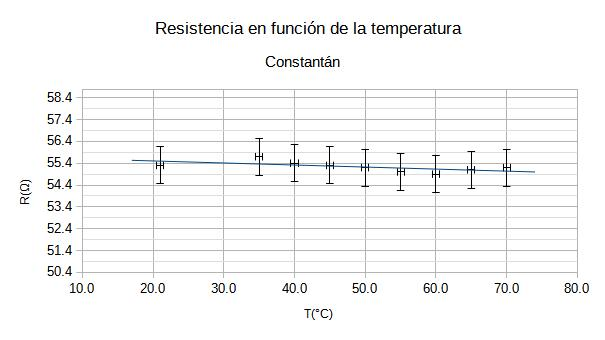
\includegraphics[width=\textwidth]{Exp1_GConst.jpg}
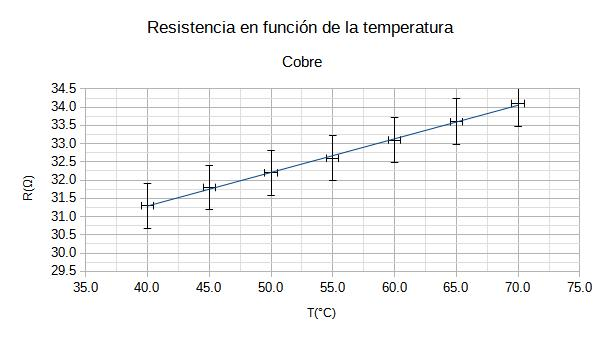
\includegraphics[width=\textwidth]{Exp1_GCobr.jpg}
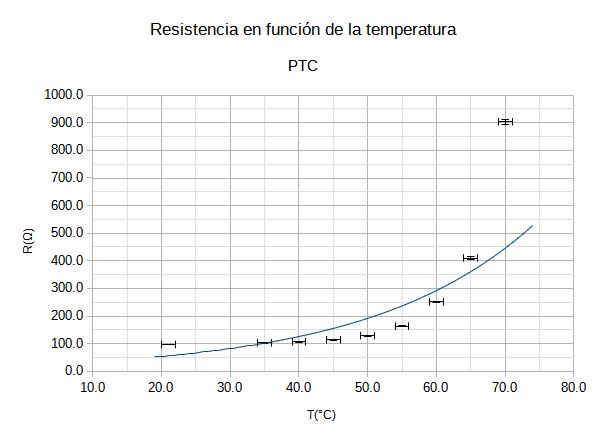
\includegraphics[width=\textwidth]{Exp1_GPTC.jpg}
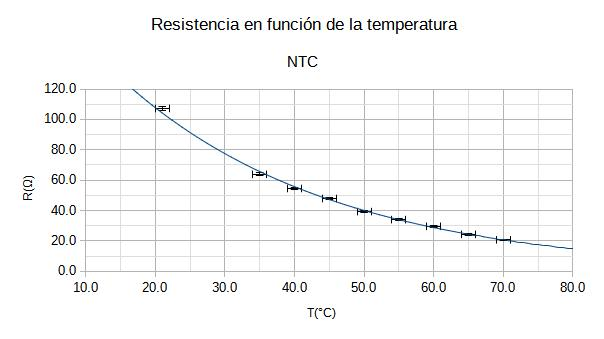
\includegraphics[width=\textwidth]{Exp1_GNTC.jpg}

En el segundo experimento, se han obtenido datos solamente para el cobre por medio de una medición indirecta: Se han medido la corriente y la tensión, y se utilizó la sencilla relación de $R = \frac{V}{I}$ para calcular la resistencia. Las incertidumbres de la voltaje y amperagen se calcularon de manera similar a lo que se hizo para los ohmímetros en la primera parte, y se utilizó la relación de que $\delta R = \sqrt{\left(\frac{\delta V}{V}\right)^2 +\left(\frac{\delta I}{I}\right)^2 } |R|$. Al final, obtenemos los siguientes datos:
\begin{table}[h!]
    \title{\textbf{Datos experimentales de la corriente, tensión, resistencia y temperatura.}}
    \centering
     \begin{tabular}{||c|c|c|c||} 
     \hline
     I(A) & V(V) & R($\Omega$) & T(°C) \\ \hline
        $0.110\pm 0.004$ & $2.280\pm 0.03$ & $20.727\pm 0.8$ & $23.200\pm 0.3$ \\ \hline
        $0.205\pm 0.005$ & $4.370\pm 0.05$ & $21.317\pm 0.6$ & $28.800\pm 0.3$ \\ \hline
        $0.300\pm 0.006$ & $6.580\pm 0.07$ & $21.933\pm 0.5$ & $36.000 \pm 0.4$\\ \hline
        $0.396\pm 0.007$ & $9.080\pm 0.09$ & $22.929 \pm 0.5$& $49.100 \pm 0.5$\\ \hline
        $0.496\pm 0.008$ & $12.000\pm 0.12$ & $24.194\pm 0.5$ & $65.300\pm 0.7$ \\ \hline
        $0.597\pm 0.009$ & $15.360\pm 0.16$ & $25.729 \pm 0.5$& $85.600 \pm 0.9$\\ \hline
        $0.699\pm 0.01$ & $19.230 \pm 0.20$& $27.511\pm 0.5$ & $107.400 \pm 1.1$\\ \hline 
     \end{tabular}
\end{table}
Finalmente, podemos representar estos datos en un gráfico para mejor visualización:

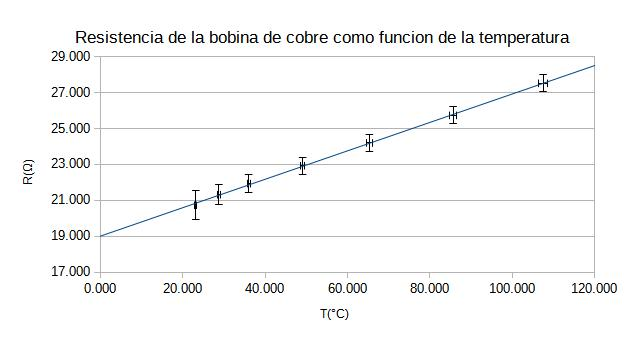
\includegraphics[width=\textwidth]{Exp1_G2.jpg}

\section{Cálculo del coeficiente de temperatura en muestras con dependencia lineal}
\subsection{Primera experiencia}
De la teoría electromagnética, podemos obtener que 
$$R = R_0\cdot(1+\alpha(T-T_0)$$
Donde, en nuestra experiencia, $T_0 = 21$°C y $R_0 = 31.4\Omega$.

Con mínimas manipulaciones, se puede obtener que $\frac{R}{R_0} = \alpha (T-T_0) + 1$. De esta manera, $\alpha$ no es más que la pendiente de la regresión lineal de $\frac{R}{R_0}$ como función de $T-T_0$. Trivialmente, $\frac{R}{R_0}$ no tiene unidades y $T-T_0$ tiene unidades de $K$, o sea, $\alpha$ tiene unidades de $K^{-1}$.

Por fín, se pueden utilizar herramientas estándar de procesamiento de datos para obtener la ecuación de la recta de mejor ajuste y representarla gráficamente:

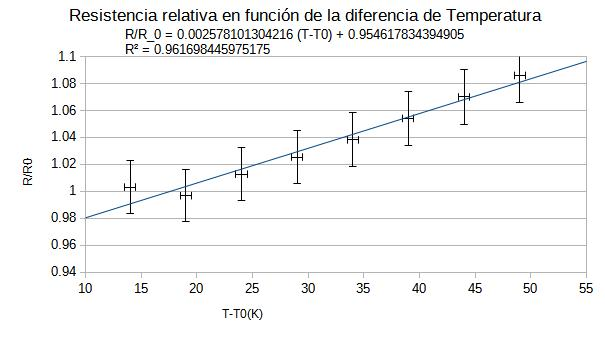
\includegraphics[width=\textwidth]{Exp1_GRegr.jpg}

Al final, se obtiene que $\alpha_1 = 2.57 10^{-3} K^{-1}$. Obviamente, es fundamental ahora propagar y calcular las incertidumbres de este valor.

Para una regresión lineal, tenemos dos fuentes de error: El estadístico, $\delta \alpha_{est}$, relacionado con la dispersión de nuestra muestra, y el instrumental, $\delta\alpha_{inst}$, relacionado con la propagación de incertidumbres de $\frac{R}{R_0}$.\footnote{\cite[62-63]{Max}}

El primero se puede calcular sin mucha dificultad:
$$\delta\alpha_{est} = |\alpha|\sqrt{\frac{r^{-2}-1}{n-2}} = 0.21\cdot 10^{-3}$$

Para el segundo, es fundamental calcular primero la incertidumbre de $\frac{R}{R_0}$:

$$\delta \frac{R}{R_0} = \frac{\delta R}{R_0} \approx 0.020$$

Y, con ella, se puede calcular el error instrumental:

$$\delta\alpha_{inst} = \sqrt{\sum_j\left[ \frac{n\cdot(T_j-T_0)-\sum_i (T_i-T_0)}{n\sum_i (T_i-T_0)^2-\left(  \sum_i (T_i-T_0)\right)^2} \right]^2\cdot\delta\frac{R}{R_0}} = 0.61 \cdot 10^{-3}$$

Y la incertidumbre total por la regla de cuadratura:

$$\delta\alpha_1 = \sqrt{\delta\alpha_{est}^2+\delta\alpha_{inst}^2} = 0.65 \cdot 10^{-3} $$

Y, con esto, se tiene el resultado final:
\begin{tcolorbox}
    \begin{equation}
        \alpha_1 = (2.6 \pm 0.7) \cdot 10^{-3} K^{-1}
    \end{equation}
\end{tcolorbox}
\subsection{Segunda experiencia}
Utilizando la exacta misma metodología de la sección anterior y aplicándola al nuevo conjunto de datos, se puede calcular $\alpha$ y su error. 

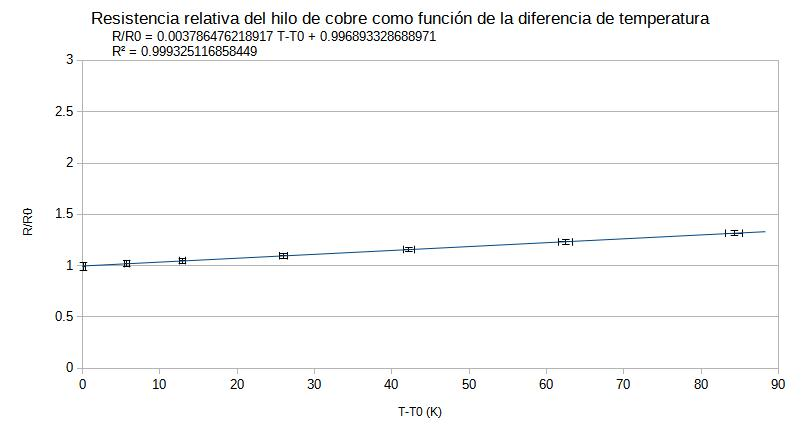
\includegraphics[width=\textwidth]{Exp1_GRegr2.jpg} 

De la regresión, se puede concluir que 
$$\alpha_2 =3.78 \cdot 10^{-3}$$
y, por el mismo procedimiento que antes, que:
$$\delta\alpha_{est} = |\alpha|\sqrt{\frac{r^{-2}-1}{n-2}} = 0.0448\cdot 10^{-3}$$
$$\delta\alpha_{inst} = \sqrt{\sum_j\left[ \frac{n\cdot(T_j-T_0)-\sum_i (T_i-T_0)}{n\sum_i (T_i-T_0)^2-\left(  \sum_i (T_i-T_0)\right)^2} \right]^2\cdot\delta\frac{R}{R_0}} =0.394 \cdot 10^{-3}$$
$$\delta\alpha_2 = \sqrt{\delta\alpha_{est}^2+\delta\alpha_{inst}^2} = 0.396\cdot 10^{-3} $$

Por fin, obtenemos un valor completamente diferente para el coeficiente de temperatura del cobre:
\begin{tcolorbox}
    \begin{equation}
        \alpha_2 = (3.8 \pm 0.4) \cdot 10^{-3} K^{-1}
    \end{equation}
\end{tcolorbox}
\subsection{Análisis de los resultados y comparación con la literatura}
Con solamente una mirada preliminar, es posible notar que hay una enorme discrepancia entre los dos resultados. Pero, si se tiene en consideración los resultados estándar de una tabla de coeficientes térmicos, el valor de $\alpha$ para el cobre debería ser $3.93\cdot 10^{-3}$ \footnote{\cite[847]{Tipler}}. De este modo, hay un error relativo, $$\frac{\alpha_1 - \alpha_{teorico}}{\alpha_{teorico}} =0.33$$ o sea, un error de 33.3\%.

Comparándolo con $\alpha_2$, que tiene un error solamente de 2.5\% en relación al esperado. Es importante mencionar también que el valor teórico de $\alpha$ está más allá de la incertidumbre calculada para $\alpha_1$, ilustrando que la medida realmente no está precisa.

Esta discrepancia se puede explicar de dos maneras distintas: La primera, y tal vez más óbvia, es que hay alguna fuente de error sistemático que no fue considerada (Algún cable mal conectado, un multimetro roto, algún problema de calibración, etc.) o, tal vez más probablemente, que el material medido no era \textit{exactamente} cobre. Dicho de otra manera, es posible que el material que medimos la resistencia estaba oxidado o distorsionado de otras maneras.

Si es el caso que la segunda explicación es válida, todos los resultados tienen bastante sentido y relativamente precisos, sin ninguna discrepancia a explicarse.

\section{Cálculo del coeficiente de activación NTC}
Con la ecuación de la resistencia de un material NTC, no podemos hacer \textit{directamente} una regresión lineal, ya que tiene forma exponencial:
$$R = R_0 \exp{\frac{Q}{k_B}\left( \frac{1}{T}-\frac{1}{T_0} \right)}$$
Donde $Q$ es la energía de activación que queremos encontrar, $k_B = 1.38\cdot 10^{-23}J/K$ y, para este caso, $T_0 = 294.2 K$ y $R_0 = 107.2 \Omega$.
Pero, con un poco de manipulación de esta ecuación y la introducción de un logarítmo, se puede hacerla tener la forma de una regresión lineal:
$$\frac{R}{R_0} = \exp{\frac{Q}{k_B}\left( \frac{1}{T}-\frac{1}{T_0} \right)}$$
$$\ln{\frac{R}{R_0}} = \frac{Q}{k_B}\left( \frac{1}{T}-\frac{1}{T_0} \right) $$

O sea, si hacemos $\ln{\frac{R}{R_0}}$ como función de $\left( \frac{1}{T}-\frac{1}{T_0} \right)$, se puede hacer una regresión lineal para encontrar $\frac{Q}{k_B}$. Utilizando las herramientas estándares de nuestro análisis, podemos obtener que
$$\frac{Q}{k_B} = 3.39\cdot 10^3$$
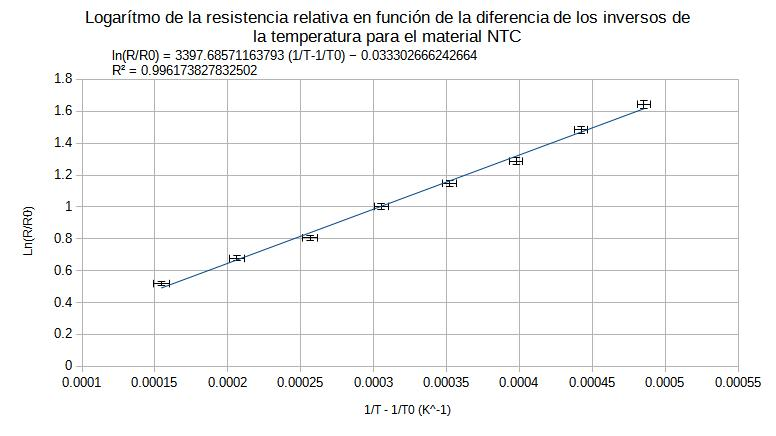
\includegraphics[width=\textwidth]{Exp1_ExpRegr.jpg}
Y, haciendo el mismo análisis de incertidumbres de antes, no olvidando que 
$$\delta\ln(\frac{R}{R_0}) = \frac{\delta \left( \frac{R}{R_0} \right)}{\frac{R}{R_0}}$$
Tenemos que 
$$\delta\frac{Q}{k_B}_{est} = |\frac{Q}{k_B}|\sqrt{\frac{r^{-2}-1}{n-2}} = 0.086\cdot 10^{3}$$
$$\delta\frac{Q}{k_B}_{inst} = \sqrt{\sum_j\left[ \frac{n\cdot\left( \frac{1}{T_j}-\frac{1}{T_0} \right)-\sum_i \left( \frac{1}{T_i}-\frac{1}{T_0} \right)}{n\sum_i \left( \frac{1}{T_i}-\frac{1}{T_0} \right)^2-\left(  \sum_i \left( \frac{1}{T_i}-\frac{1}{T_0} \right)\right)^2} \right]^2\cdot\delta\ln{\frac{R}{R_0}} = 0.0531 \cdot 10^{3}}$$
$$\delta\frac{Q}{k_B}= \sqrt{\delta\frac{Q}{k_B}_{est}^2+\delta\frac{Q}{k_B}_{inst}^2} = 0.0101 \cdot 10^{3} $$

De esta manera, podemos trivialmente calcular $Q$, ya que 
$$Q = k_b \cdot \left( \frac{Q}{k_B} \pm \delta\frac{Q}{k_B} \right)$$
\begin{tcolorbox}
    \begin{equation}
        Q = (4.69 \pm 0.02) \cdot 10^{-20} J = (0.293 \pm 0.001) eV
    \end{equation}
\end{tcolorbox}

Resultado que es una fracción de un electrón-vóltio, orden de magnitud correcta para las energías de activación. De esta manera, se atingen todos los objetivos del experimento con éxito.

\printbibliography
\end{document}
